\chapter{The Sensory Afferent Database}\label{ch:database}
\graphicspath{{D:/Github/Bipedal_Robot/Documentation/Reports and Papers/Dissertation/Figures/50-database/}{figs/50-database/}}

\section{A Structured Afferent Resource}\label{sec:sadb_resource}

The synthetic nervous system of Chapter~\ref{ch:sns} is assembled from physiological parts: Ia, Ib, and II afferents, the reflex pathways they drive, and the spinal circuits those pathways modulate. Building that controller is a design problem, and design needs parameters, not only principles. For each sensory channel, the designer has to know what the receptor encodes, over what ranges of length, velocity, and force it operates and with what receptor dynamics, and what the afferent does at the spinal end: which interneuron populations it contacts, whether the action is excitatory or inhibitory, whether the target is ipsilateral or contralateral, and in which phase of the step cycle the pathway is open. Every element of that specification was established experimentally, one pathway and one preparation at a time, across a century of work in cat, mouse, rat, and human preparations, and the results are distributed over an enormous primary literature. A controller designer is not the only reader stranded by that scatter. An animal researcher planning the next experiment wants to know which preparations established a pathway property, and how the property compares across species, before committing a preparation to it. A roboticist wants to know which receptor encoding a sensor should imitate. Those readers ask different questions of the same literature, and the literature answers none of them without being gathered, structured, and searchable first.

Reviews assemble part of this knowledge, but none can serve as the working resource itself. The three this dissertation draws on illustrate both the value and the limit: \citet{van_de_crommert_review_1998} organize the sensory control of the central pattern generator around the treadmill-training literature, \citet{windhorst_muscle_2007} assigns functional roles to muscle proprioceptive feedback within a broader argument about spinal networks, and \citet{windhorst_spinal_2022} weighs accumulated spinal-circuit model assumptions against the experimental record. Each synthesizes a slice of the literature; none can be filtered by afferent class, animal preparation, or pathway, none carries its demonstrating papers as attached and followable evidence, and each is fixed at its publication date. Extracting gain ranges, receptor dynamics, and phase-dependent feedback roles from reviews organized around a hypothesis means redoing the literature search the review was meant to spare the reader. When this work began, no structured compilation of afferent properties existed from which a controller designer, an animal researcher, or a roboticist could draw them; every reader redid the same search.

The Sensory Afferent Database (SADb) was built within the AARL's NeuroNex Communication, Coordination, and Control in Nervous Systems (C3NS) effort to close that gap, and we presented it at Neuroscience 2023 \citep{bolen_sensory_2023}. It is a database rather than a bibliography: each paper carries distilled mechanism notes, each sensory feedback pathway is a first-class record linked to the papers that established it, and each computational model of afferent control is linked to its source paper and to the pathway records it implements. The database lives in a five-table Airtable base (Papers, Feedback, Models, Review Papers, and Recorders) backed by the laboratory's Zotero libraries, with the DOI as the canonical identifier for every record.

This chapter and the controller chapter are therefore built as one program. The database informs the sensory channels of Chapter~\ref{ch:sns}: the afferent classes the controller monitors, the signal encoding each channel carries, and the connection rules its circuit implements all trace to records held here, and Section~\ref{sec:sadb_use} documents that mapping. The sections that follow describe how the corpus was assembled, audited, pruned, and packaged into its present form.

Methods

The audit and curation effort reported here began from a three-way reconciliation, because the database's three homes did not agree. The author's personal Zotero collection held 538 items, the AARL group library's Biology subtree held 911 items across 27 collections, and the Airtable base held 99 papers. Matching record by record on DOI and normalized title showed that the personal collection was essentially a subset of the group library (all 483 personal DOIs present) and that the Airtable base was a small curated subset rather than a mirror: 95 of its 99 papers resolved to records in the group library's Biology subtree, while 443 personal items had never been entered at all. The gap was imported in verified batches, with every written record re-read and checked after writing, bringing the Papers table to 532 records. The corpus then kept growing while curation caught up: citation mining in the style of Research Rabbit contributed a Crossref-verified digest of recent papers, newly saved references flowed in from the laboratory's Zotero libraries, and a bulk pass imported 372 papers auto-classified from the laboratory's staged collection of PDFs. By the close of the expansion the audited corpus stood at 943 papers, the full set against which every later decision in this chapter was made.

Curation then proceeded under rules designed to make every note citable. A note is written from the paper's own text, from the abstract at minimum and from the full text when available, never from the curator's recollection of the paper; papers for which no text could be found were logged and left bare rather than guessed. Notes are one to three sentences of distilled mechanism, following the template of the laboratory's earliest records, and free-text fields are constrained by controlled vocabularies for animal preparations and afferent classes. Each feedback pathway is named by a fixed grammar of afferent, action, side, joint, and phase (for example, ``Ib stance to swing''), so that pathway records compose into circuits the way the controller will use them. Ambiguous cases were flagged for a human ruling rather than decided silently.

The final curation wave added the fields that make the corpus answerable as a database: afferent class, animal-study potential, robot-and-simulation translation notes, and prune status fields, together with a corpus citation graph exposed as record-to-record links. Drafting was machine-assisted at scale, with 374 papers curated in fifteen batches; every batch passed automated vocabulary, abstract-paste, and duplicate gates before anything was written, and every record was verified against its grounding text after the write. Grounding remained the binding constraint throughout. A PDF-first rule recovered grounding for 47 of 55 flagged papers from the laboratory's own library, and a university-authenticated browser session recovered abstracts for 24 of the 70 papers that had no findable text; the rest stayed bare by rule.

Pruning followed, in three stages, each approved before execution, and together the stages removed 436 records: 382 papers, close to four hundred, plus 54 orphaned review, model, and pathway records that lost their anchors to the paper cuts. First, 95 records left as off-topic or orphaned: 88 papers removed as satellite topics (machine-learning and aerodynamics methods, flow sensing without neurophysiology, and fish swimming biomechanics), as duplicates, or as isolated records stranded by an earlier strict flagging pass, plus seven orphaned pathway, model, and review records. Second, a cut list of 290 papers assembled from explicit rules for duplicates, monographs, and conference abstracts, and from a weighted rubric ranking the remainder by citation count, age, rating, network isolation, and record thinness, while 351 protected records (foundational authors, feedback-linked papers, highly cited work, and pre-1940 classics) were excluded from consideration. Third, a final round removed four papers and 47 review records whose links had been emptied by the earlier cuts. The prune was deliberate on two grounds. The working base had swollen past the laboratory's free-plan 1,000-record cap, and a curated resource that answers a design question in ten records beats a haystack of a thousand; the audit had shown the corpus contained both, and the satellite material was answering nothing. No record was destroyed: every deletion was snapshotted, and the packaged explorer described below carries the 382 cut papers under an archived flag, so the audited corpus remains reconstructible in full.

The audit and the prune are also why the laboratory built its own explorer app rather than adopting an existing tool. Airtable remains the working home of the data, but it is a curation tool, not a reader: it cannot travel past the laboratory's account, and a flat grid answers none of the questions this corpus exists to answer. An off-the-shelf bibliometric viewer was tried first and retired within weeks; it drew one crowded picture of the whole corpus, offered no drill-through from a cluster to the papers inside it, and let a handful of mega-cited classics dominate every view. The query patterns this resource must serve are specific: filter by afferent class, animal preparation, or pathway; follow a pathway record to the papers that established it in each species; walk the citation neighborhood of a candidate anchor paper; count the corpus by any two dimensions at once. A circuit designer wiring a reflex, an animal researcher choosing a preparation, and a roboticist choosing a sensor analog ask different questions of the same records, and no existing tool answered any of them. The corpus itself was therefore packaged as a laboratory tool: a single-file, offline explorer embedding the audited corpus, the citation graph, and the named clusters, with searchable and pivotable tables, focus-mode citation neighborhoods drawn in the laboratory's own convention of papers as neurons with excitatory and inhibitory synapses, and a generated knowledge base with an index page plus cluster, pathway, afferent, and animal pages, all distributed as a zip that runs in a browser on any machine with no network connection.

\section{Audited Corpus and Curation Coverage}\label{sec:sadb_corpus}

At the close of the curation effort the working base held 957 records: 561 papers, 39 feedback-pathway records, 244 model records, 109 review records, and 4 recorder entries, 43 records below the laboratory's 1,000-record operating cap, with room to grow. Coverage of the retained papers is concentrated where the laboratory's design and experimental work needs it. Of the 561 retained papers, 523 carry curation notes, 426 carry animal-preparation tags, 240 carry notes assessing each paper's animal-study potential, 118 are linked to named feedback pathways, 86 carry an afferent classification, and 258 carry notes translating the paper's findings toward robot or simulation use; 550 carry DOIs, and 38 remain bare pending a findable text.

The citation graph was built over the full audited corpus of 943 papers, which includes the 382 records the prune later removed and which the packaged database retains under an archived flag. Within that corpus, 730 papers are connected by 11,130 directed in-corpus citation pairs, and a Louvain community partition of the graph resolves 18 named topic clusters, from the classics of afferent locomotor control and spinal interneuron circuit modeling through human balance and posture to bioinspired flow sensing and deep-learning methods. The partition earned its keep in the prune: the satellite clusters it exposed, the flow-and-flight sensing, fish swimming, and neural-network method clusters, match the topic groups the first prune stage removed. Within that audited corpus, 833 papers carry curation notes and 318 carry attached PDFs, and the prune's 382 removed records remain in the package under an archived flag so the audited scope stays reconstructible in full. The corpus, its citation graph, its cluster assignments, and the flat corpus export are distributed together in the packaged explorer, and Figure~\ref{fig:sadb_explorer} shows its table view as packaged. Figure~\ref{fig:sadb_clusters} summarizes the same corpus at the topic-cluster level: the seven clusters the curated corpus retains, and the satellite clusters the prune removed in full.

\begin{figure}[htbp]
\centering
\includegraphics[width=\textwidth]{sadb_explorer.png}
\caption[The SADb Explorer offline corpus tool]{The SADb Explorer, the packaged offline interface to the audited corpus, shown on its table view: the Papers table sorted by citation count, with the tag column recording each paper's curation state, animal preparation, and afferent or pathway links. The application runs in a browser from a single file with no network connection required.}
\label{fig:sadb_explorer}
\end{figure}

\begin{figure}[htbp]
\centering
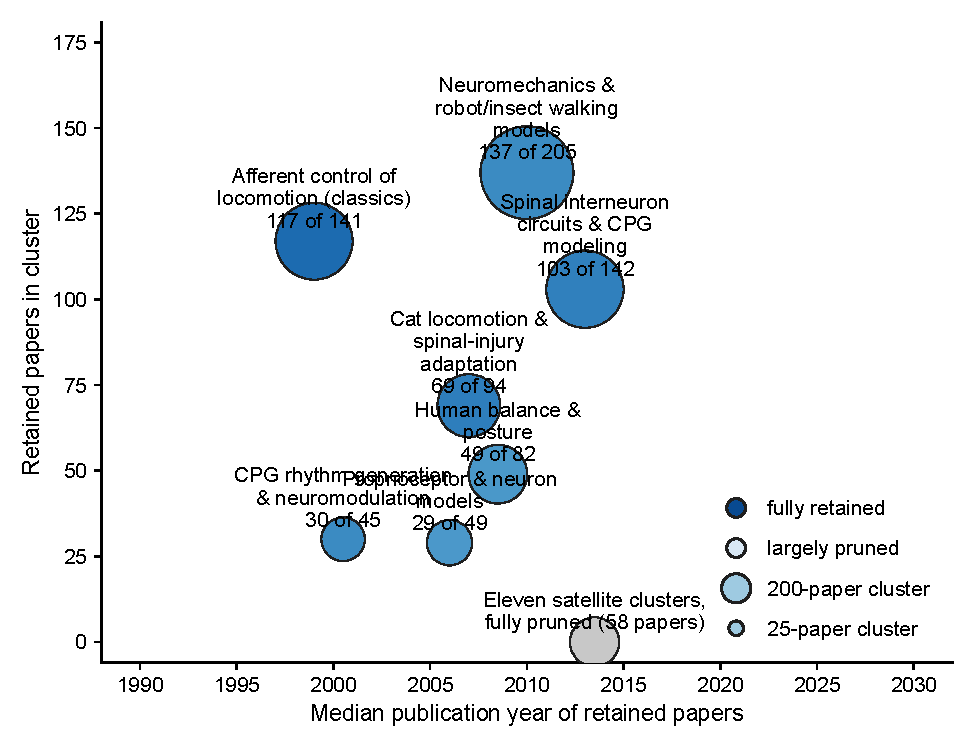
\includegraphics[width=0.92\textwidth]{sadb_clusters.pdf}
\caption[Citation-graph topic clusters of the audited corpus]{The Louvain topic clusters of the audited corpus, one bubble per cluster. Horizontal position is the median publication year of the cluster's retained papers, vertical position the number of retained papers, and bubble area the audited cluster size; darker fill marks a larger retained fraction. The seven clusters with retained papers form the curated core, from the afferent-control classics and spinal-circuit modeling to neuromechanics and robot walking; the gray bubble aggregates the eleven satellite clusters the prune removed in full (58 papers), among them the fish-swimming, flow-and-flight-sensing, and neural-network-method clusters of the prune account. 27 of the 561 retained papers fall outside the citation-graph partition.}
\label{fig:sadb_clusters}
\end{figure}

\section{AI-Assisted Literature Triage}\label{sec:sadb_triage}

Expanding a curated corpus is dominated by triage: deciding, paper by paper, what a record is about and whether it belongs. We evaluated AI tools for this task in a comparative study presented at Neuroscience 2024 \citep{bolen_using_2024}. The evaluation found the expected trade: the tools accelerated the population of the database, but their output still required substantial human oversight for accuracy.

The curation workflow reported here is the operational answer to that finding, a division of labor in which the machine drafts and the human rules. The machine contributed scale: batch drafting from grounded text, automated gates that rejected abstract pastes and duplicate records before writing, and per-record verification after it. The gates earned their place on caught failures, including a record that shipped another paper's abstract under its title until the grounding pass flagged it. The human held every decision that required judgment or carried risk: the curation vocabulary and its amendments, the 164 flagged judgment calls surfaced for ruling, and every single deletion in the prune, each stage of which waited for explicit approval. The gates and flags are not ceremony; they are the oversight the 2024 evaluation showed was necessary, made concrete.

\section{Toward Robot and Simulation Use}\label{sec:sadb_use}

The database exists to feed the sensorium of Chapter~\ref{ch:sns}. Its pathway records enumerate the signal taxonomy the controller's sensory channels implement: Ia afferents carrying length and velocity, Ib afferents carrying force, II afferents carrying length, and contact receptors marking the stance--swing boundary (Section~\ref{sec:preliminary_sim_methods}); Table~\ref{tab:sadb_afferents} summarizes what the corpus establishes for each class. The pathway naming grammar maps directly onto circuit edges, since a record's afferent class fixes the signal encoding, its phase fixes the gating, and its action fixes the sign, so translating a pathway record into a controller connection is a lookup rather than a literature search; Table~\ref{tab:sadb_pathways} lists the principal pathway records with the papers that demonstrate them. The Models table carries the lineage the controller instantiates, from the two-level rhythm-generator and pattern-formation architecture \citep{rybak_modelling_2006} through muscle-reflex walking \citep{geyer_musclereflex_2010} to the two-layer neuromechanical walker the laboratory's controller descends from \citep{deng_neuromechanical_2019}, and the 258 robot-and-simulation translation notes exist precisely to shorten the step from paper to wiring decision. Figure~\ref{fig:sadb_pivot} shows the two-dimension count the explorer's pivotable tables produce over the retained corpus, the afferent classes against the animal preparations: the classical cat preparation carries the largest share of the Ia, Ib, II, and cutaneous records, and the arthropod records enter through the mechanosensory class.

\begin{table}[htbp]
\caption{Afferent classes represented in the Sensory Afferent Database, the signal each class carries, and the pathway roles the corpus records for it. Anchor references are corpus papers linked to the corresponding records; the signal summary for the Ia, II, and Ib rows follows the ensemble afferent recordings of \citet{prochazka_ensemble_1998}.}
\label{tab:sadb_afferents}
\begin{tabularx}{\textwidth}{@{}lllX@{}}
\toprule
\textbf{Class} & \textbf{Receptor} & \textbf{Signal carried} & \textbf{Recorded pathway roles (anchors)} \\
\midrule
Ia & muscle spindle primary & muscle length and velocity & homonymous stretch excitation \citep{eccles_integrative_1958}; reciprocal inhibition of the antagonist pool \citep{jankowska_effect_1967} \\
II & muscle spindle secondary & static muscle length & midlumbar disynaptic relay onto motor nuclei \citep{edgley_interneuronal_1987}; stance-phase support of extensor activity \citep{mazzaro_afferent_2006} \\
Ib & Golgi tendon organ & whole-muscle force & autogenic inhibition at rest, stance-phase reversal to excitation, and the load gate on swing onset \citep{dietz_significance_2000, dominguez_candidate_2020} \\
III/IV & free nerve endings & metabolic and nociceptive signals, converging with cutaneous and group II--III afferents as flexor-reflex afferents & phase-dependent resetting of the locomotor rhythm \citep{schomburg_flexor_1998} \\
Cutaneous & skin and foot-pad receptors & contact and perturbation events & flexor excitation and phase-modulated stance correction \citep{sherrington_flexion_1910, forssberg_stumbling_1979} \\
\bottomrule
\end{tabularx}
\end{table}

\begin{figure}[htbp]
\centering
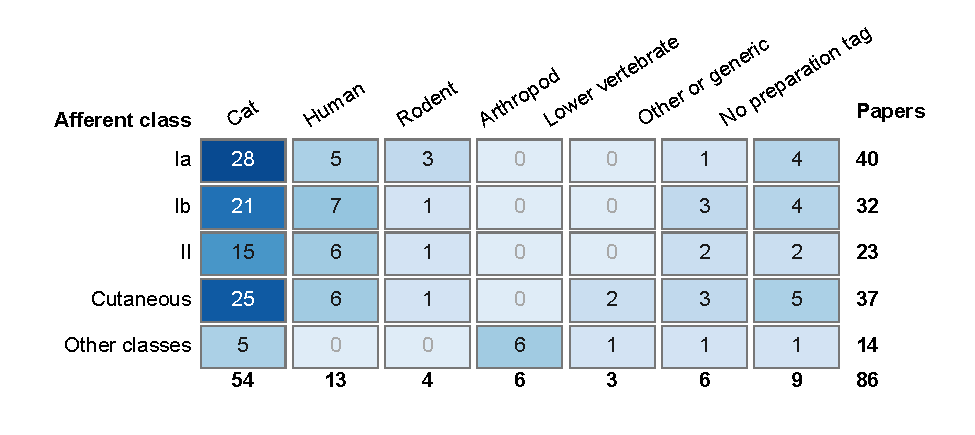
\includegraphics[width=0.96\textwidth]{sadb_pivot.pdf}
\caption[Corpus pivot by afferent class and preparation]{A two-dimension pivot over the retained corpus, of the kind the explorer's pivotable tables produce. Rows are afferent classifications and columns animal preparations; each cell counts the retained papers carrying both tags, so a paper with several preparations or classes counts once in each corresponding cell, and the margins count unique papers. The base is the 86 retained papers that carry an afferent classification, of which 9 have no preparation tag.}
\label{fig:sadb_pivot}
\end{figure}

\begin{sidewaystable}[p]
\caption{Principal feedback-pathway records of the database's Feedback table, named by the fixed grammar of afferent, action, and phase. Linked papers are counted over the full audited corpus of 943 papers; for every pathway listed, the count is unchanged under the retained corpus of 561. Demonstrating references are the corpus papers linked to each record, as curated in the database.}
\label{tab:sadb_pathways}
\fontsize{10pt}{12pt}\selectfont
\begin{tabularx}{\textheight}{@{}llXrp{0.26\textheight}@{}}
\toprule
\textbf{Pathway record} & \textbf{Class} & \textbf{Recorded action in the step cycle} & \textbf{Linked papers} & \textbf{Demonstrating references} \\
\midrule
Ia monosynaptic excitation & Ia & stretch excitation of the homonymous motor pool, with the pathway gain modulated over the step cycle & 7 & \citep{eccles_integrative_1958, capaday_amplitude_1986} \\
Ia reciprocal inhibition & Ia & inhibition of the antagonist motor pool through the Ia inhibitory interneurons, rhythmically active in fictive locomotion & 6 & \citep{jankowska_effect_1967, pratt_ia_1987} \\
Ib disynaptic inhibition & Ib & autogenic non-reciprocal group I inhibition of the loaded muscle's own pool, reduced during stance & 5 & \citep{jankowska_common_1981, stephens_short_1996} \\
Ib disynaptic excitation & Ib & the locomotor reversal: group I input excites synergist extensor pools during the extensor phase, replacing the resting inhibition & 6 & \citep{mccrea_disynaptic_1995, pearson_enhancement_1998} \\
Ib stance to swing & Ib & the load gate: Ib input from ankle extensors prolongs stance, so swing is not initiated while the leg is loaded & 17 & \citep{dietz_significance_2000, dominguez_candidate_2020} \\
Ia or II stance to swing & Ia, II & flexor-length gate on stance termination: lengthening of flexor muscles in late stance ends extension and resets the cycle & 10 & \citep{hiebert_contribution_1996, akay_degradation_2014} \\
type II excitatory & II & stance-phase support of ankle-extensor activity through the midlumbar group II relay & 5 & \citep{edgley_interneuronal_1987, mazzaro_afferent_2006} \\
Cutaneous flexor excitation & Cutaneous & flexion withdrawal and the stumbling corrective reaction, phase-modulated over the cycle & 16 & \citep{sherrington_flexion_1910, forssberg_stumbling_1979} \\
\bottomrule
\end{tabularx}
\end{sidewaystable}

The 39 pathway records extend beyond the mammalian core of Table~\ref{tab:sadb_pathways}: paired excitation and inhibition records cover the chordotonal organs and trochanteral hair plates of insect legs, a load-feedback record covers the campaniform sensilla, and further records hold fictive locomotion without sensory feedback (12 linked papers), group III/IV fatigue, and one paper each for somatosensory, vestibular, and visual contributions to postural control. The controller of Chapter~\ref{ch:sns} implements the mammalian subset.

The corpus also reaches ahead to the sensorium extensions planned in Section~\ref{sec:fw_senses}. The human balance and posture cluster and the multisensory recalibration cluster are the entry points for the vestibular and ocular feedback work, already curated and already connected to the locomotor core through the citation graph. The knowledge base makes this reach practical for new students as well: the cluster, pathway, and animal pages compress a literature that took months to curate into an onboarding document measured in pages, and the animal pages let an experimentalist start from a preparation rather than a topic.

The honest accounting is that the resource is deeper than it is broad in places. The afferent classification covers 86 of 561 retained papers, concentrated in the pathway-rich core rather than spread across the corpus, and the flagged vocabulary gaps (vestibular and visual preparations among them) mark where the classification must grow before the extensions of Section~\ref{sec:fw_senses} can be wired from the database alone. The growth policy follows from the prune: additions should be substantive records or clearly flagged stub twins, never bare rows, so that the corpus that the controller work, the next experiments, and the next students inherit stays as searchable as the one this chapter documents.
